\documentclass[11pt]{article}

\usepackage{helvet}
\renewcommand{\familydefault}{\sfdefault}

\usepackage{amsmath,amssymb,amsthm}
\usepackage{graphicx}
\usepackage{subfigure}
\usepackage{caption}

\usepackage[top=1in,bottom=1in,left=1in,right=1in]{geometry}
\usepackage{paralist}

\usepackage[pagebackref=true,colorlinks=true,breaklinks=true,linkcolor=blue,citecolor=blue,urlcolor=blue]{hyperref}

\usepackage{fancyhdr}
\setlength{\headheight}{15.2pt}
\pagestyle{fancyplain}
\lhead[RUI]{RUI} 
\chead[hTeXML: Web Authoring for STEM]{SHORT\_RUNNING\_TITLE}
\rhead[C. Aguilar]{C. Aguilar}

% Move sections heading to the center
\usepackage[center]{titlesec}
\titleformat{\section}[hang]{\normalfont\scshape}{\thesection.}{.5em}{\filcenter}[]
\titleformat{\subsection}[hang]{\normalfont\scshape}{\thesubsection.}{.5em}{\filcenter}[]

% Changes title of bibliography
\renewcommand\refname{\textbf{\Large References}}

%=========================================================
\begin{document}

\begin{center}
\textbf{\Large Project Description}\\[0.25cm]
\hrulefill\\[0.25cm]
\textbf{\Large Facilitating the Creation of Open Educations Resources \\[1ex] for STEM Educators}\\
\hrulefill
\end{center}
\baselineskip 1.5em

%=========================================================
\section{Introduction}
The term \textbf{open educational resources} (OER) was first coined in 2002 by a panel of academics convened by UNESCO to discuss the OpenCourseWare initiative by MIT \cite{oerguidelines}.  At the center of the OER initiative is the belief that educational resources should be available at no-cost to students and that teaching and learning is strengthened when teaching resources are shared openly by educators. What are open educational resources?  As defined by UNESCO \cite{oerworldcongress}, OER are ``teaching, learning, and research materials in any medium that
\begin{enumerate}[(i)]
\item reside in the public domain or
\item have been released under an open license that permits no-cost access, use adaptation, and redistribution by others with no or limited restrictions.
\end{enumerate}
David Wiley from Lumen Learning expands on part (ii) of the definition as the permission to engage in the so-called \textbf{5R} activities \cite{wileynd}:
\begin{enumerate}[(i)]
  \item Retain - make, own, and control a copy of the resource
  \item Revise - edit, adapt, and modify your copy of the resource
  \item Remix - combine your original or revised copy of the resource with other existing material to create something new
  \item Reuse - use your original, revised, or remixed copy of the resource publicly
  \item Redistribute - share copies of your original, revised, or remixed copy of the resource with others.
\end{enumerate}

In legal terms, the ``open'' in OER rely on copyright licenses that allow users to engage in the 5R activities.  A frequently used open license is one of six possible \textbf{Creative Commons} (CC) licenses\footnote{\href{https://creativecommons.org/about/cclicenses/}{https://creativecommons.org/about/cclicenses/}} (others exist such as the GNU Free Documentation License\footnote{\href{https://www.gnu.org/licenses/fdl-1.3.en.html}{https://www.gnu.org/licenses/fdl-1.3.en.html}}).  A subset of the CC licenses are designed to allow users of creative content, such as textbooks, to freely distribute, \textbf{adapt}, \textbf{remix}, and \textbf{build upon} the content in any medium or format, possibly for commercial use, provided attribution is given to the original creator.  Open-access or freely available textbooks are sometimes confused with OER but the difference is that the former type of resources may not permit a user the right to distribute, remix, or adapt the work.

Aside from the financial savings of OER for students, other benefits of OER include the ability to customize the content to meet the needs of students, the ability to share the content with other educators, giving students first-day access to course materials which research shows improves learning outcomes \cite{LA:2017}, and the flexibility of engaging with the course materials when and where students choose or are able to.  In particular, for students in urban areas that use public transit to get to school, the ability to access course materials on a mobile device is a significant benefit \cite{CC:17, MS:14} over traditional hard-copy textbooks.

Recent studies show that awareness of OER in colleges and universities has grown in the last decade due in large part by statewide and/or institutional initiatives.  For example, in annual national surveys conducted by Bay View Analytics, which collects a representative sample of the broad range of teaching faculty in U.S. higher education, 46\% of polled faculty indicated being aware of both OER and CC licensing in the 2021-2022 survey compared to only 17\% in 2014-2015 \cite{JS-JS:2022}; see Figure~\ref{fig:oer-awareness}.
\begin{figure}
\centering
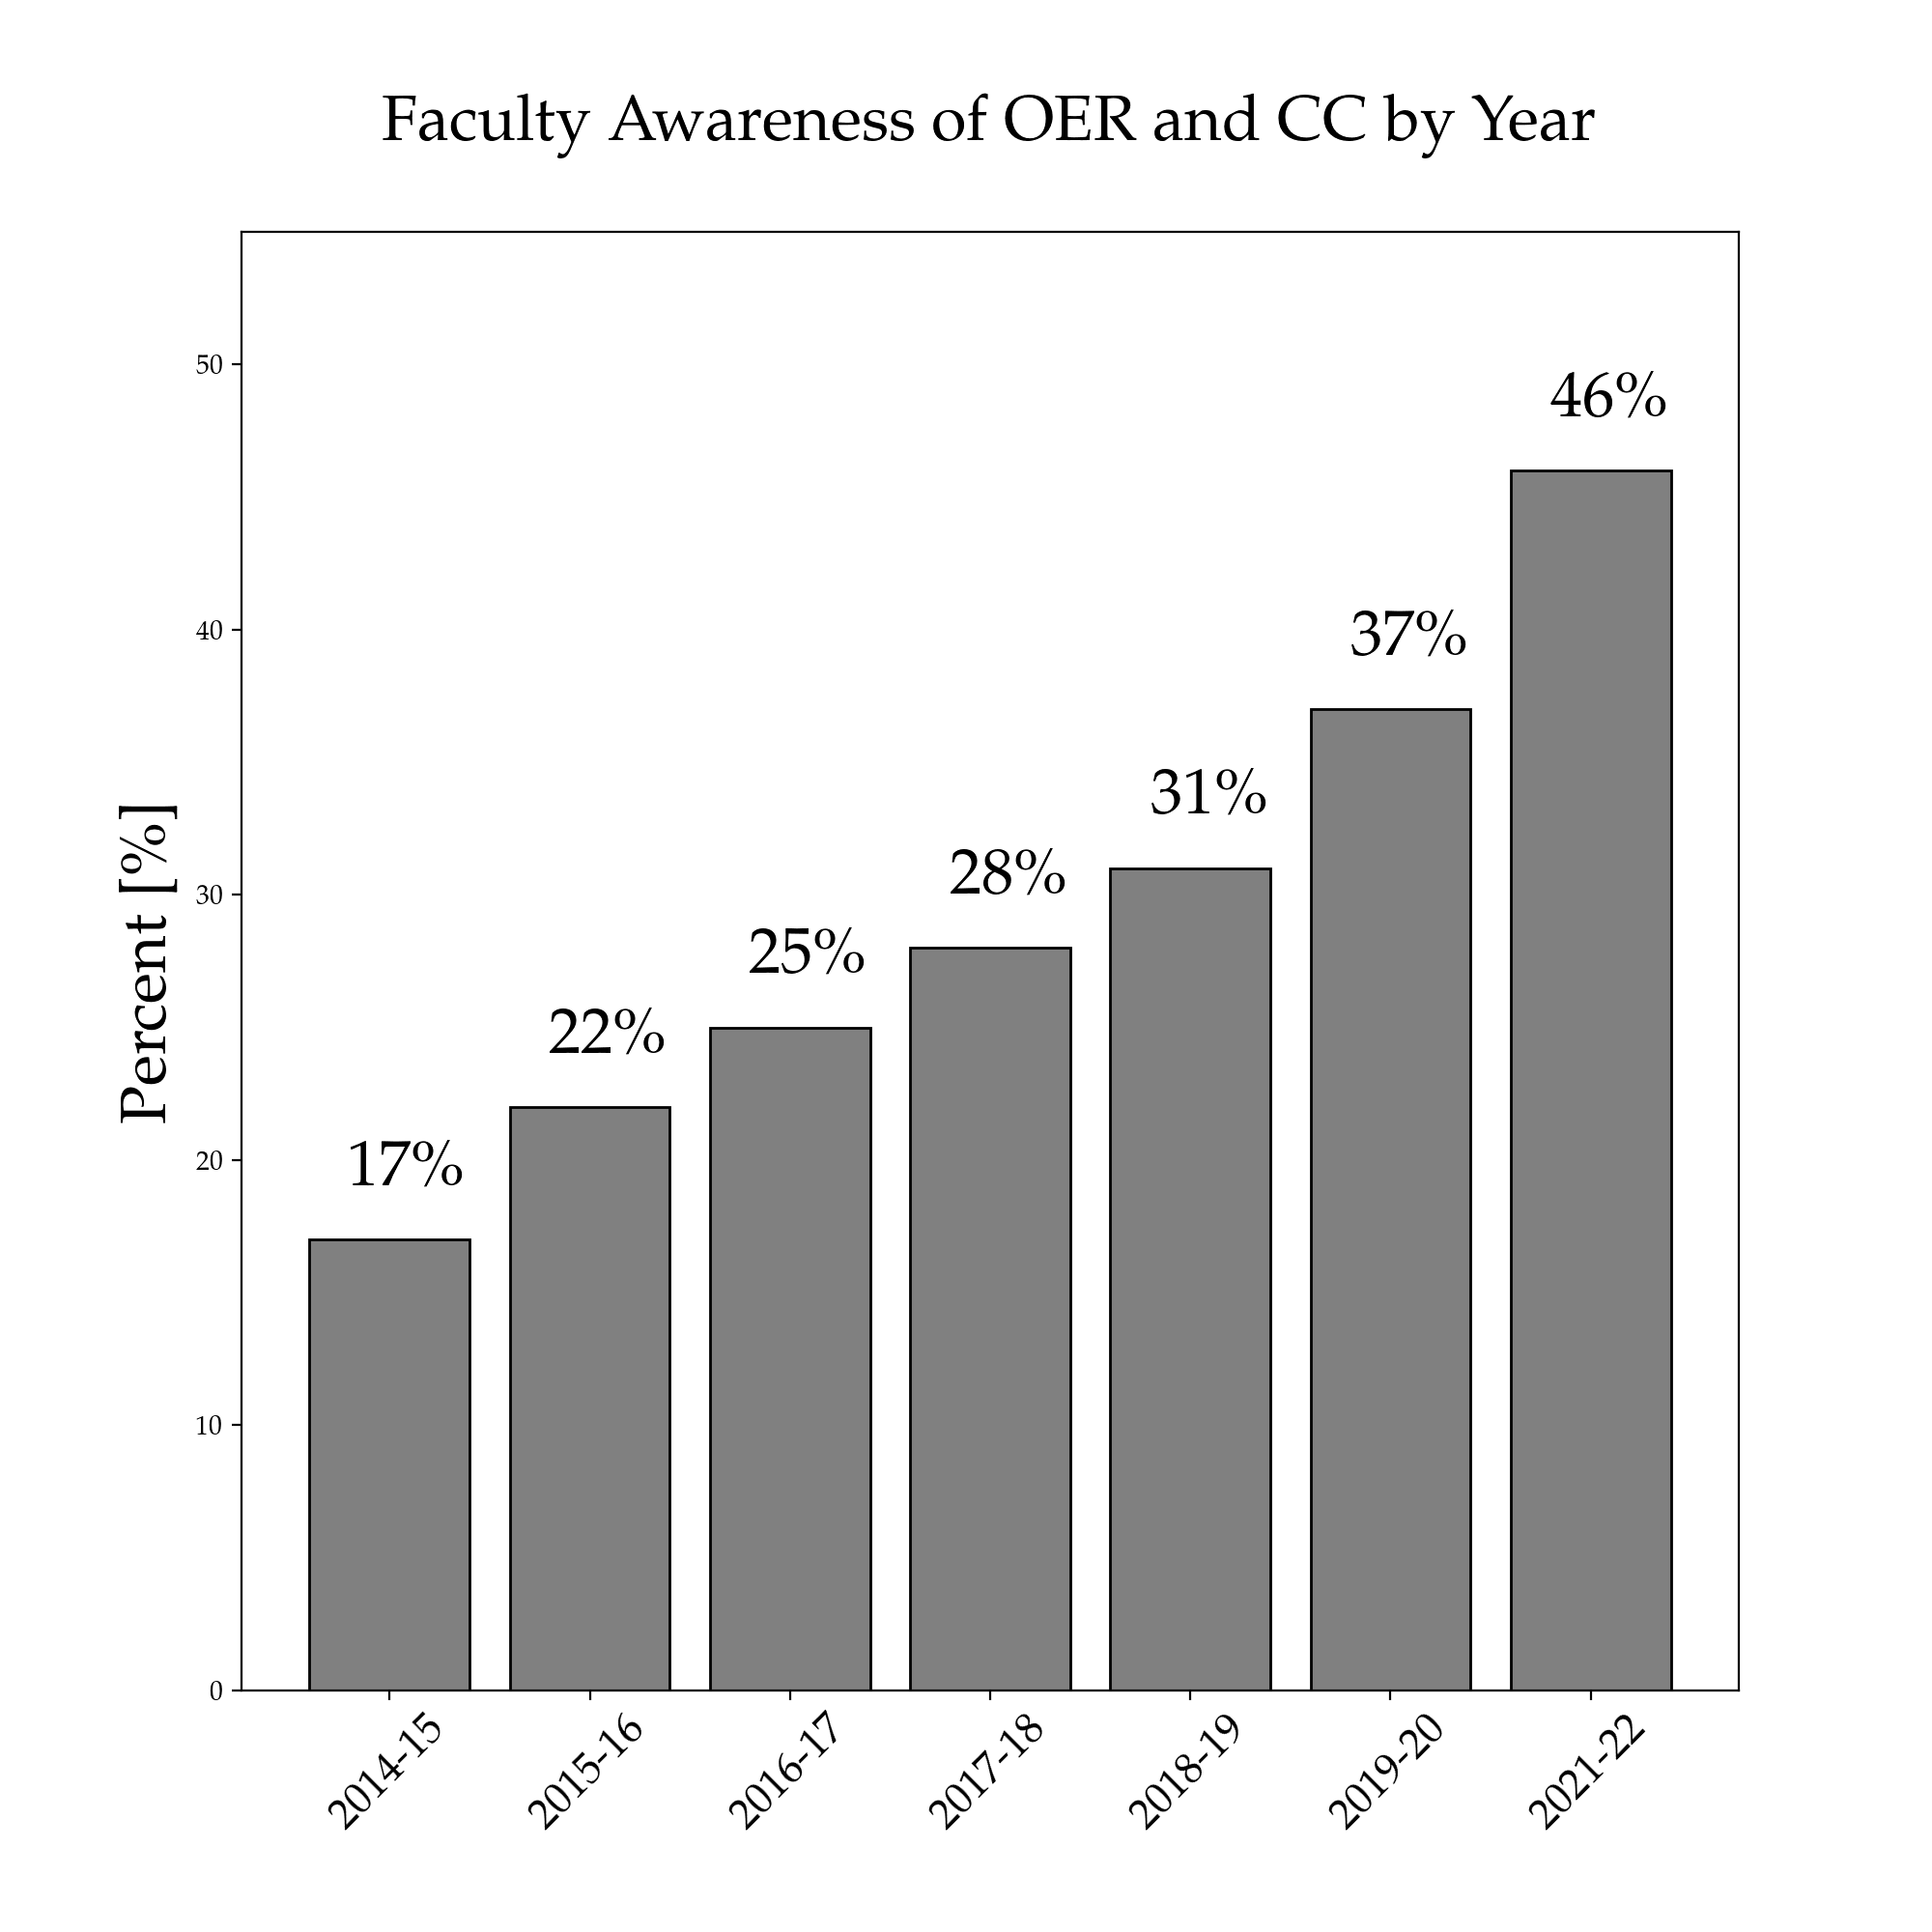
\includegraphics[width=90mm]{oer_awareness.png}
\caption{The percent of U.S. higher education teaching faculty who indicated being aware of open educational resources (OER) and Creative Commons licenses by year \cite{JS-JS:2022}.}
\label{fig:oer-awareness}
\end{figure}
In the same survey \cite{JS-JS:2022}, the majority of respondents indicated that, because of the switch to online learning due to the COVID pandemic, their opinions of online learning improved (54\%) as did their acceptance of digital materials (68\%).  Although progress has been made in increasing college faculty awareness of OER, much work remains to be done to increase the actual usage and creation of quality open educational resources \cite{flvc2022}.

\subsection{Cost of College Textbooks: Relief on the Horizon?}
According to data collected and made publicly available by the U.S. Bureau of Labor Statistics (BLS), the price of college textbooks from 2000-2022 has increased by an average of 6\% annually which is nearly 3 times the average annual inflation rate of 2\% over the same period \cite{bls}. In the blog posts \cite{perry2018, perry2022}, economist Mark J. Perry of the University of Michigan\textendash Flint published other selected consumer price index data for several goods and services over the same period; the only two services that saw an increase in price higher than college textbooks were hospital services and college tuition \cite{perry2018, perry2022}; see Figures~\ref{fig:cpi-textbooks-2018}-\ref{fig:cpi-textbooks-2022}. In early 2017, the price of college textbooks began to flattened and then began to decline moderately in 2019 and 2020, remaining flat in 2021 and now experiencing increases throughout 2022.
\begin{figure}[t]
\begin{minipage}[t]{8.0cm}
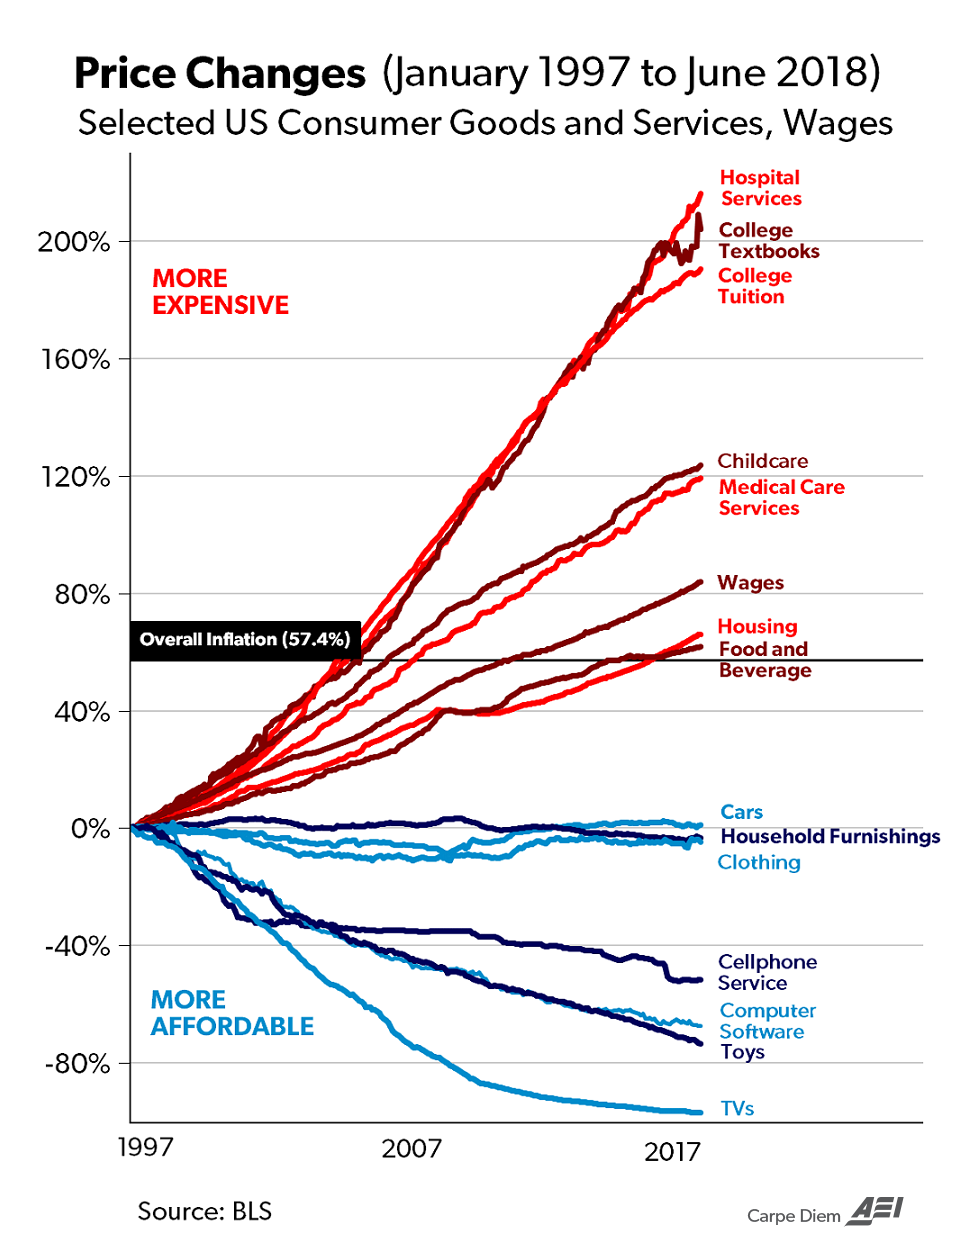
\includegraphics[width=70mm,height=80mm]{cpichart2018a.png}
\caption{\small From January 1997 to June 2018, the price of college textbooks has increased by approximately 204\%. (source: \href{aei.org/carpe-diem}{aei.org/carpe-diem}) }\label{fig:cpi-textbooks-2018}
\end{minipage}
\hfill
\begin{minipage}[t]{8.0cm}
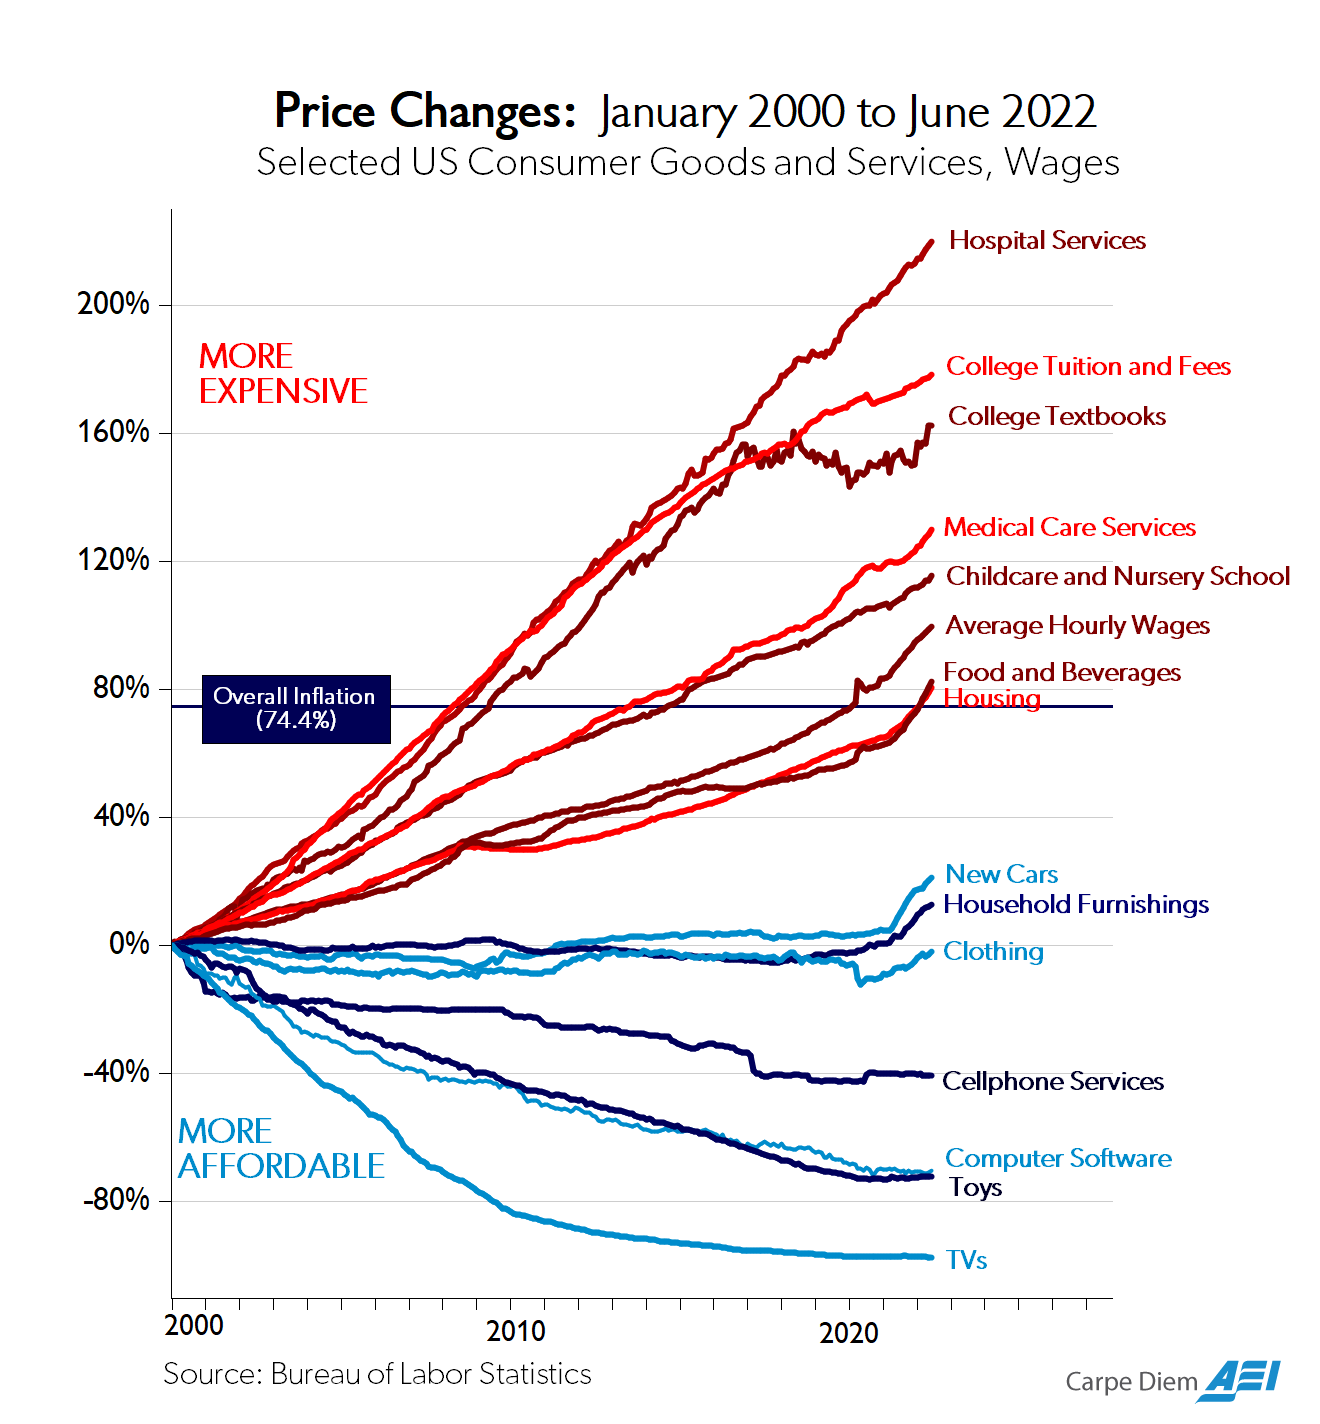
\includegraphics[width=70mm,height=82mm]{cpi2022junea-3.png}
\caption{\small From January 2000 to June 2022, the price of college textbooks has increased by approximately 162\%. (source: \href{aei.org/carpe-diem}{aei.org/carpe-diem})}\label{fig:cpi-textbooks-2022}
\end{minipage}
\end{figure}

Despite the moderate decrease in college textbooks prices in recent years, textbook prices remain a substantial burden for students.  In a series of broadly cited surveys conducted by the Florida Virtual Campus on students from Florida's public colleges and universities (FLVC)\footnote{Surveys were conducted by FLVC in 2010, 2012, 2016, 2018, and 2022; the 2020 survey was cancelled due to the COVID pandemic.}, more than half (53.5\%) of all 13,000 respondents in 2022 reported that they had not purchased a required textbook due to its cost \cite{flvc2022} (In 2018, of the 22,000 respondents, 66.6\% reported the same.).  Other key findings of the 2022 survey found that the high cost of textbooks caused students to:
\begin{itemize}
\item taking fewer courses (43.7\%),
\item not register for a specific course (38.5\%),
\item earn a poor grade due to not being able to afford the textbook (32.4\%), and
\item dropped out of a course (24.2\%).
\end{itemize}
Moreover, students in bachelor degree programs were more likely to spend over \$300 per term on textbooks compared to graduate students or students pursuing an associates degree.

\subsection{Technological Barriers of OER}
Despite the growing number of educators and institutions embracing the usage of OER in teaching and learning, the actual usage of OER is still somewhat limited, see for instance \cite{MB:2022} and references therein.  More importantly, even in communities where OER are adopted, the rights of users to engage in the 5R activities are often hampered by technological barriers \cite{SO:19}.

Here will talk about the number of math books that do not have source latex/html in the repositories \href{https://open.umn.edu/opentextbooks}{Open Textbooks Library} and \href{https://openstax.org/}{OpenStax} 

%=========================================================
\section{Project Proposal}



\subsection{Overview}

%=========================================================
\subsection{Existing Technology}

\subsubsection{MathML}
\textbf{Mathematical Markup Language} (MathML) is a language used to describe the presentation and content of mathematical notation.  MathML is used in web browsers, in computer algebra systems (CAS), print typesetting, and voice synthesis.  The goal of MathML is to enable mathematically rich documents on the web in the same way that HTML has enabled this functionality for text; MathML markup can be written alongside HTML markup.  MathML markup can become quite complicated even for simple mathematical expressions.  As an example, the MathML markup to describe the mathematical expression
\[
x = \frac{-b \pm\sqrt{b^2-4ac}}{2a}
\]
is given by
\begin{verbatim}
    <math>
      <mi>x</mi><mo>=</mo>
      <mfrac>
        <mrow>
          <mo>-</mo><mi>b</mi><mo>&pm;</mo>
          <msqrt>
            <msup><mi>b</mi><mn>2</mn></msup>
            <mo>-</mo><mn>4</mn><mi>a</mi><mi>c</mi>
          </msqrt>
        </mrow>
        <mrow><mn>2</mn><mi>a</mi></mrow>
      </mfrac>
    </math>
\end{verbatim}
whereas the equivalent LaTeX markup is
\begin{verbatim}
    \[
        x = \frac{-b \pm \sqrt{b^2-4ac}}{2a}
    \]
\end{verbatim}
Needless to say, typing MathML by hand can be very tedious and error prone and as such it is not intended to be edited by hand.  Instead, the generation of MathML markup is usually the task of specialized equation editors or the result of a conversion from another markup language such as LaTeX.
 
\subsubsection{LaTeX2HTML}
\textbf{LaTeX2HTML} is a command line utility that converts LaTeX documents to web pages in HTML (latex2html.org).  As described on the programs website, ``\textit{LaTeX2HTML replicates the basic structure of a LaTeX document as a set of interconnected HTML files which can be explored using automatically generated navigation panels. The cross-references, citations, footnotes, the table of contents and the lists of figures and tables, are also translated into hypertext links. Formatting information which has equivalent tags in HTML (lists, quotes, paragraph breaks, type styles, etc.) is also converted appropriately. The remaining heavily formatted items such as mathematical equations, pictures or tables are converted to images which are placed automatically at the correct positions in the final HTML document''.}\footnote{latex2html.org}  Although LaTeX2HTML's goal of converting LaTeX documents to web pages is similar in spirit to htexml, there are core design features that distinguish LaTeX2HTML and htexml, such as:

\begin{itemize}
\item Documentation for LaTeX2HTML is scarce and not easily accessible for an average computer user.  Basic usage of LaTeX2HTML is not available on the projects website or github page.
\item LaTeX2HTML's conversion of mathematical equations to images to be rendered by the browser is in conflict with the goal of creating mathematically rich documents on the web that are rendered natively by the browser.
\item LaTeX2HTML is written in \textbf{perl} and must be installed from source using using configure, make, and make install or is available as a package for Linux or through the MacOS package manager Homebrew.
\item After installation, the program is available as a command line utility whereas all the functionality of htexml is accessible from a browser.
\item Even for an experienced computer user, installing LaTeX2HTML from source or via Homebrew can present its challenges that could discourage users from using the program.  htexml requires no installation.
\end{itemize}

\subsubsection{TeX4ht}
\textbf{TeX4ht} is a command line tool that converts LaTeX documents to various output formats including HTML, ODT (open document format), or DocBook.  According to the programs documentation, modern TeX distributions such as TeX Live and Miktex come with TeX4ht and a related bundling tool called \textbf{make4ht}.  



%=========================================================
\subsection{Placeholder}


%=========================================================
\section{Research Plan and Timeline}


\noindent\textbf{First Year:}  

\noindent\textbf{Second Year:}  

\noindent\textbf{Third Year:}  
%=============================================
\section{Broader Impacts}

\subsection{Research Impact}


%=============================================
\subsection{Training of STEM Students}

\subsection{Educational Impact}    


%=============================================
\newpage

% Bibliography
\begin{thebibliography}{99}

  \bibitem{LA:2017} Agnihotri, L., Essa, A., \& Baker, R. (2017, March). Impact of student choice of content adoption delay on course outcomes. {\em In Proceedings of the Seventh International Learning Analytics \& Knowledge Conference} (pp. 16-20)

  \bibitem{MB:2022} Baas, M., van der Rijst, R., Huizinga, T., van den Berg, E., Admiraal, W. (2022). Would you use them? A qualitative study on teachers' assessments of open educational resources in higher education. {\em The Internet and Higher Education}, 54, 100857.

  \bibitem{CC:17} Cooney, C. (2017). What impacts do OER have on students? Students share their experiences with a health psychology OER at New York City College of Technology. {\em International Review of Research in Open and Distributed Learning}, 18(4), 155-178.

  \bibitem{oerguidelines} Miao, F., Mishra, S., Orr, D., \& Janssen, B. (2019). Guidelines on the development of open educational resources policies. {\em UNESCO Publishing}.\newline \href{https://unesdoc.unesco.org/ark:/48223/pf0000371129}{https://unesdoc.unesco.org/ark:/48223/pf0000371129}

  \bibitem{oerworldcongress} UNESCO (2017), Second World OER Congress: Ljubljana OER Action Plan.\newline \href{https://unesdoc.unesco.org/ark:/48223/pf0000260762}{https://unesdoc.unesco.org/ark:/48223/pf0000260762}

  \bibitem{wileynd} Wiley, D. (n.d.). Defining the ``open'' in open content and open educational resources.\newline \href{http://opencontent.org/definition/}{http://opencontent.org/definition/}.

  \bibitem{JS-JS:2022} J.E. Seaman, J. Seaman (2022). Turning Point for Digital Curricula: EducationAL Resources in U.S. Higher Education. {\em Bay View Analytics}. \newline \href{https://www.bayviewanalytics.com/reports/turningpointdigitalcurricula.pdf}{https://www.bayviewanalytics.com/reports/turningpointdigitalcurricula.pdf}

  \bibitem{JS-JS:2018} Seaman, J.E., Seaman, J. (2002). Freeing the Textbook: Educational Resources in U.S. Higher Education. {\em Bay View Analytics}.\newline \href{https://www.bayviewanalytics.com/reports/freeingthetextbook2018.pdf}{https://www.bayviewanalytics.com/reports/freeingthetextbook2018.pdf}

  \bibitem{SO:19} Ovadia, S. (2019). Addressing the Technical Challenges of Open Educational Resources.  {\em portal: Libraries and the Academy}, 19(1), 79-93. \href{http://doi.org/10.1353/pla.2019.0005}{http://doi.org/10.1353/pla.2019.0005}

  \bibitem{bls} U.S. Bureau of Labor Statistics, {\em Consumer Price Index for All Urban Consumers: College textbooks in U.S. city average}, Series ID CUUR0000SSEA011, \href{https://data.bls.gov/cgi-bin/srgate}{https://data.bls.gov/cgi-bin/srgate}

  \bibitem{perry2018} Perry, M.J. (2018). The CD `chart of the Century' Makes the Rounds at the Federal Reserve. {\em Carpe Diem}. \href{https://www.aei.org/carpe-diem/the-chart-of-the-century-makes-the-rounds-at-the-federal-reserve/}{https://www.aei.org/carpe-diem/the-chart-of-the-century-makes-the-rounds-at-the-federal-reserve/}.

  \bibitem{perry2022} Perry, M.J. (2022). Chart of the Day \ldots or Century?. {\em Carpe Diem}. \href{https://www.aei.org/carpe-diem/chart-of-the-day-or-century-8/}{https://www.aei.org/carpe-diem/chart-of-the-day-or-century-8/}.

  \bibitem{MS:14} Smale, M.A., \& Regalado, M. (2014). Commuter students using technology. {\em EDUCAUSE Review Online}. Retrieved from \href{http://www.educause.edu/ero/article/commuter-students-using-technology}{http://www.educause.edu/ero/article/commuter-students-using-technology}

  \bibitem{flvc2022} Florida Virtual Campus, 2022 Student Textbook and Instructional Materials Survey. Tallahassee, FL. \href{https://dlss.flvc.org/colleges-and-universities/research/textbooks}{https://dlss.flvc.org/colleges-and-universities/research/textbooks}.

\end{thebibliography}


\end{document}
